\section{Overview on Development Setup}

A setup for development is explained in table~\ref{tab:requirements}. The most basic components are 
required for hands-on development. Main issue is a python interpreter and common libaries.\footnote{For example
cherrypy, pyserial and optionally a module for SQL-bindings in Python.}

Figure~\ref{setupic} shows the last version of the used development system. The keyboard and monitor on the host machine
is just used to monitor debug output and use the included \textsl{interactive} mode on the \textsc{WSN}.\footnote{So you can 
type in commands meant for nodes on the host machine instead of using the RESTful http-access}

\ref{nodepic} and \ref{hostpic} show the expected results after a clean startup. The controller identifies itself with a
self-chosen name and exchanges basic data for database population.
 

\begin{table}[h] 
\centering 
\begin{tabular}{|l||l|} 
General Component & Specific Component\\ 
\hline 
i86 host machine & 300MHz, 512MB\\ 
host OS & Debian stable(Squeeze) \\ 
Python Interpreter & Python 2.7 with pyserial \\ 
Database & MySQL\footnote{A local sqlite version with reduced functionality has no additional requirements} \\ 
1 Wireless Sensor Node as Controller & Renesas ZMD28-BRD \\
n Wireless Sensor Node as Client & Renesas ZMD28-BRD \\ 
\end{tabular} 
\caption{ Table of Requirements} 
\label{tab:requirements} 
\end{table}


\begin{figure}[h]
   \centering
   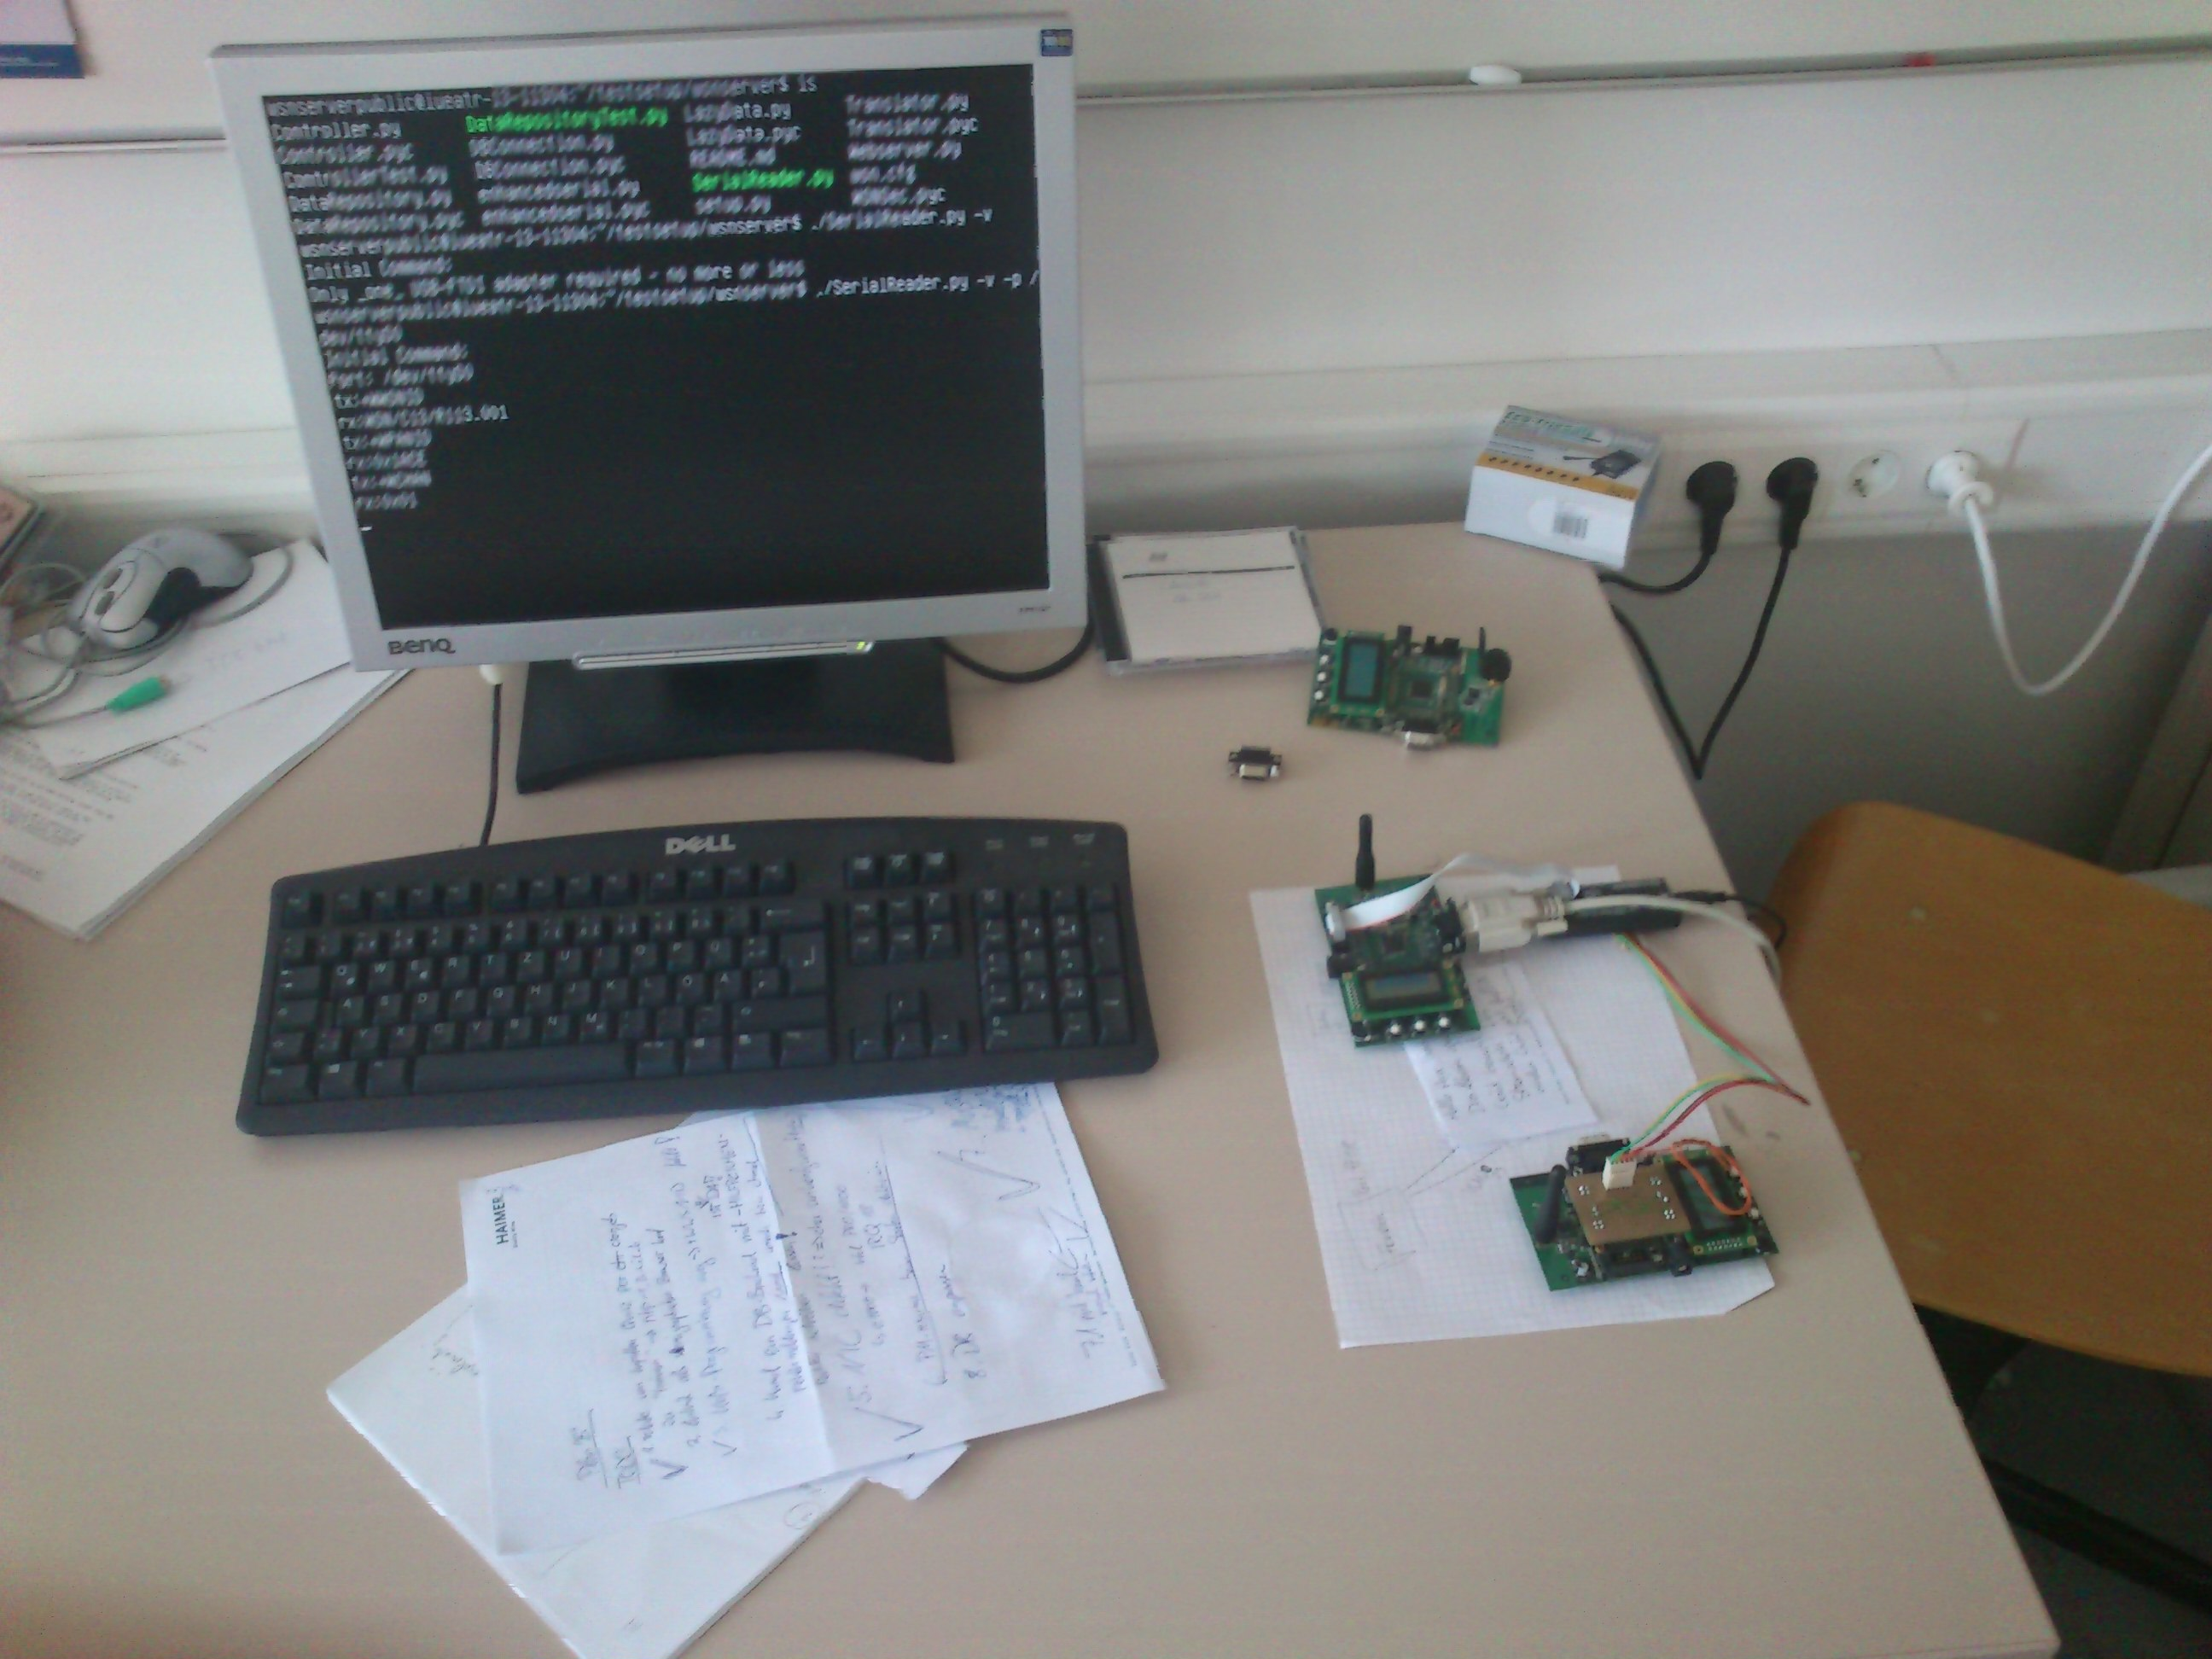
\includegraphics[width=0.8\textwidth]{pic/whole_setup.jpg}%
   \caption{Glimpse on the development setup}
   \label{setupic}%
\end{figure}

-low cost iso available at XXX

\begin{figure}[h]
   \centering
   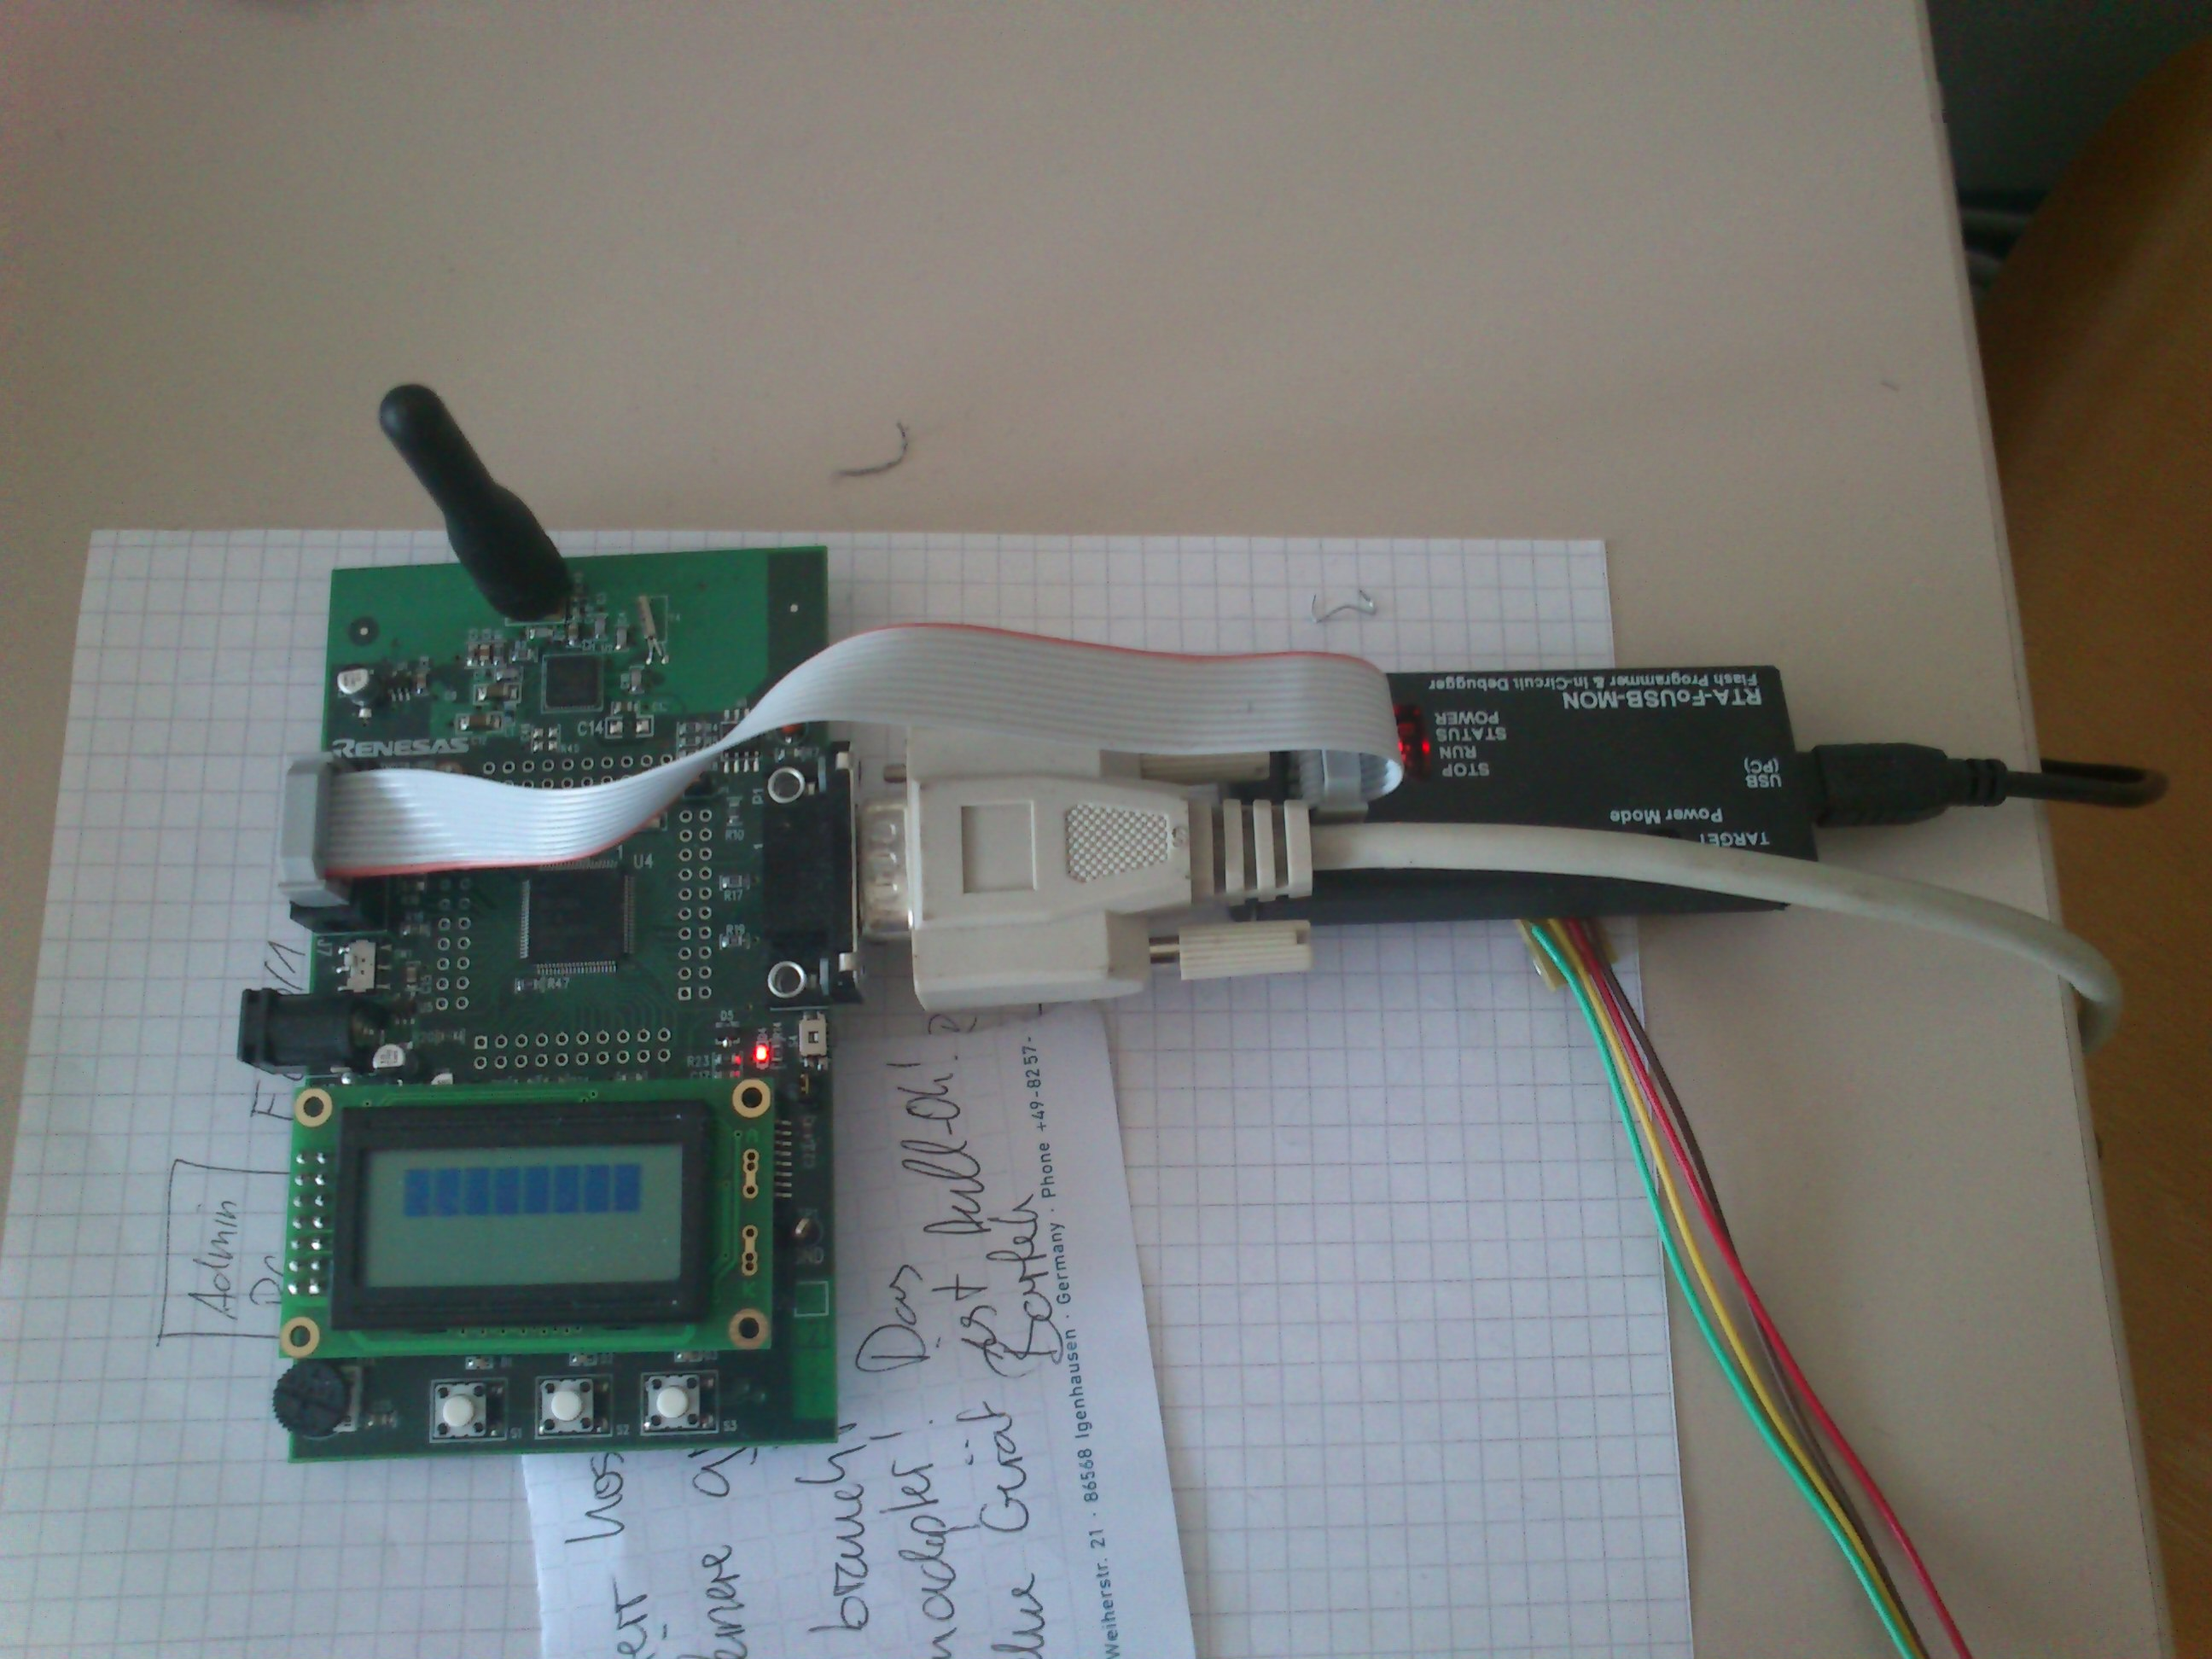
\includegraphics[width=0.8\textwidth]{pic/controller.jpg}%
   \caption{Renesas Node with Custom Programming and Serial Connector}
   \label{nodepic}%
\end{figure}

- less nodes as focused on communication

\begin{figure}[h]
   \centering
   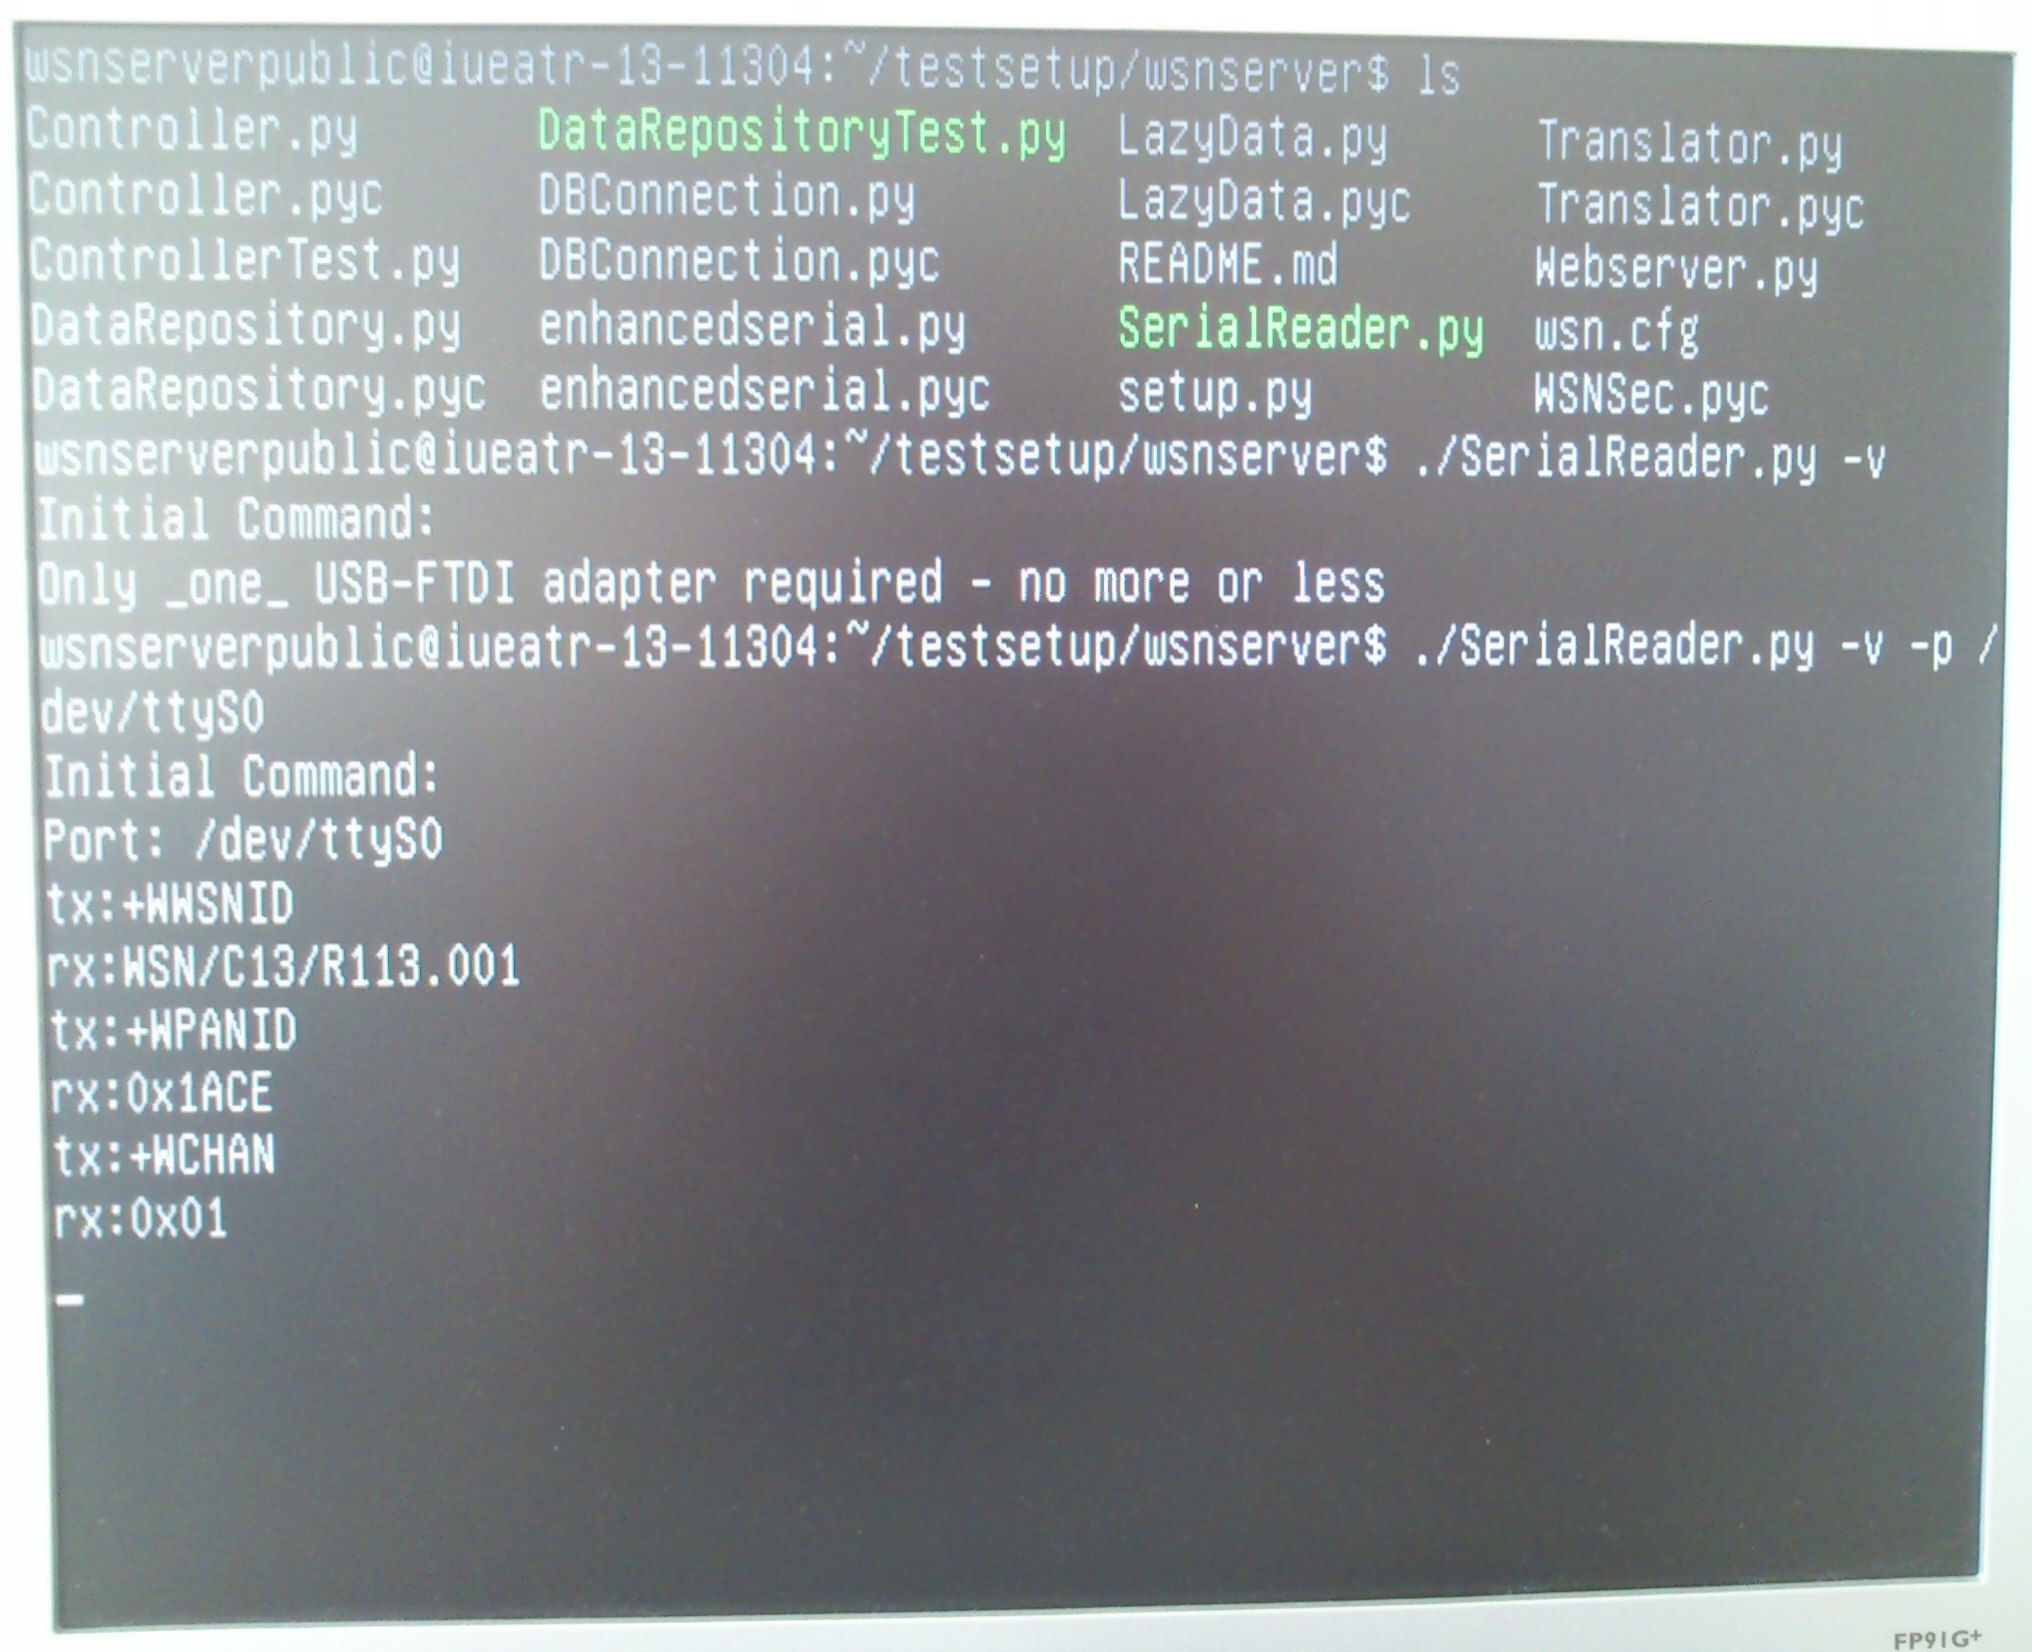
\includegraphics[width=0.8\textwidth]{pic/host_machine.jpg}%
   \caption{Console Output on Host Machine}
   \label{hostpic}%
\end{figure}

- initialisiation description

